\documentclass{article}
\usepackage[utf8]{inputenc}
\usepackage{multicol}
\usepackage{listings}
\usepackage{verbatim}
\usepackage{color}
\usepackage{geometry}

\usepackage{float}
\usepackage{amsmath}
\usepackage{hyperref}
\setlength{\belowcaptionskip}{-10pt}
\setlength{\abovecaptionskip}{-30pt}
\floatstyle{boxed} 
\restylefloat{figure}
\usepackage{graphicx}
\definecolor{codegreen}{rgb}{0,0.6,0}
\definecolor{codegray}{rgb}{0.5,0.5,0.5}
\definecolor{codepurple}{rgb}{0.58,0,0.82}
\definecolor{backcolour}{rgb}{0.95,0.95,0.92}

\lstdefinestyle{mystyle}{
	backgroundcolor=\color{backcolour},   
	commentstyle=\color{codegreen},
	keywordstyle=\color{blue},
	numberstyle=\tiny\color{codegray},
	stringstyle=\color{codepurple},
	basicstyle=\footnotesize,
	breakatwhitespace=false,         
	breaklines=true,                 
	captionpos=b,                    
	keepspaces=true,                 
	numbers=left,                    
	numbersep=5pt,                  
	showspaces=false,                
	showstringspaces=false,
	showtabs=false,                  
	tabsize=2
}

\lstset{style=mystyle}
\title{Data Mining\\
		Home work 04\\Descriptive Statistics}
\author{Aqeel Labash\\ \textbf{Supervisor:} Jaak Vilo}
\date{17 February 2016}
\geometry{
	a4paper,
	total={170mm,257mm},
	left=10mm,
	top=5mm,
}
\begin{document}
	\maketitle
	\section*{First Question}
	The things that I took home is :) :
	\begin{enumerate}
\item  Each data type has it's own
\item When we want to compare data to each other it's always better for the plot of the groups to be more scalable for people eyes.
\item If we are using line width to show information , there should be a fixed max width.
\item When using color for categories, the max number we should use is 6-12 color , otherwise the reader will get lost between the color's.
\item It's better to use separable channels for different abstract dimensions.
\item There is no bad or good way to show data, but it should match our goal.
\item Using 3d visualization should be accompanied with extra caution.Because what we think it's more clear may delay the information delivery.
\item In 3d visualization the depth take away ability of comparison because of perspective distortion.
\item When we have complex changes it's better to use series of visualization rather than animation because we lose track of global changes and focus on local changes.
\item Validate against the right threat.
	\end{enumerate}
	\section*{Second Question}
While trying to plot I found an outliers or damaged data (height , weight less than zero ) there was about 3472 row. I cleaned them using the following code:
\begin{lstlisting}[language=R]
#### Second Question ######
ncmp = read.csv('ncmp_1415_final_non_disclosive.csv',header = TRUE)
nrow(ncmp[ncmp$height<0,])
ncmp <- ncmp[ncmp$height>0,]
\end{lstlisting}
\textbf{Note:}The data later changed on the homework page with clean data, anyway I sticked to this data since I already started with it.
In the following figure I plotted the requested combination (age,height,bmi,age) while showing the gender in colors.
\begin{figure}[H]
\begin{center}
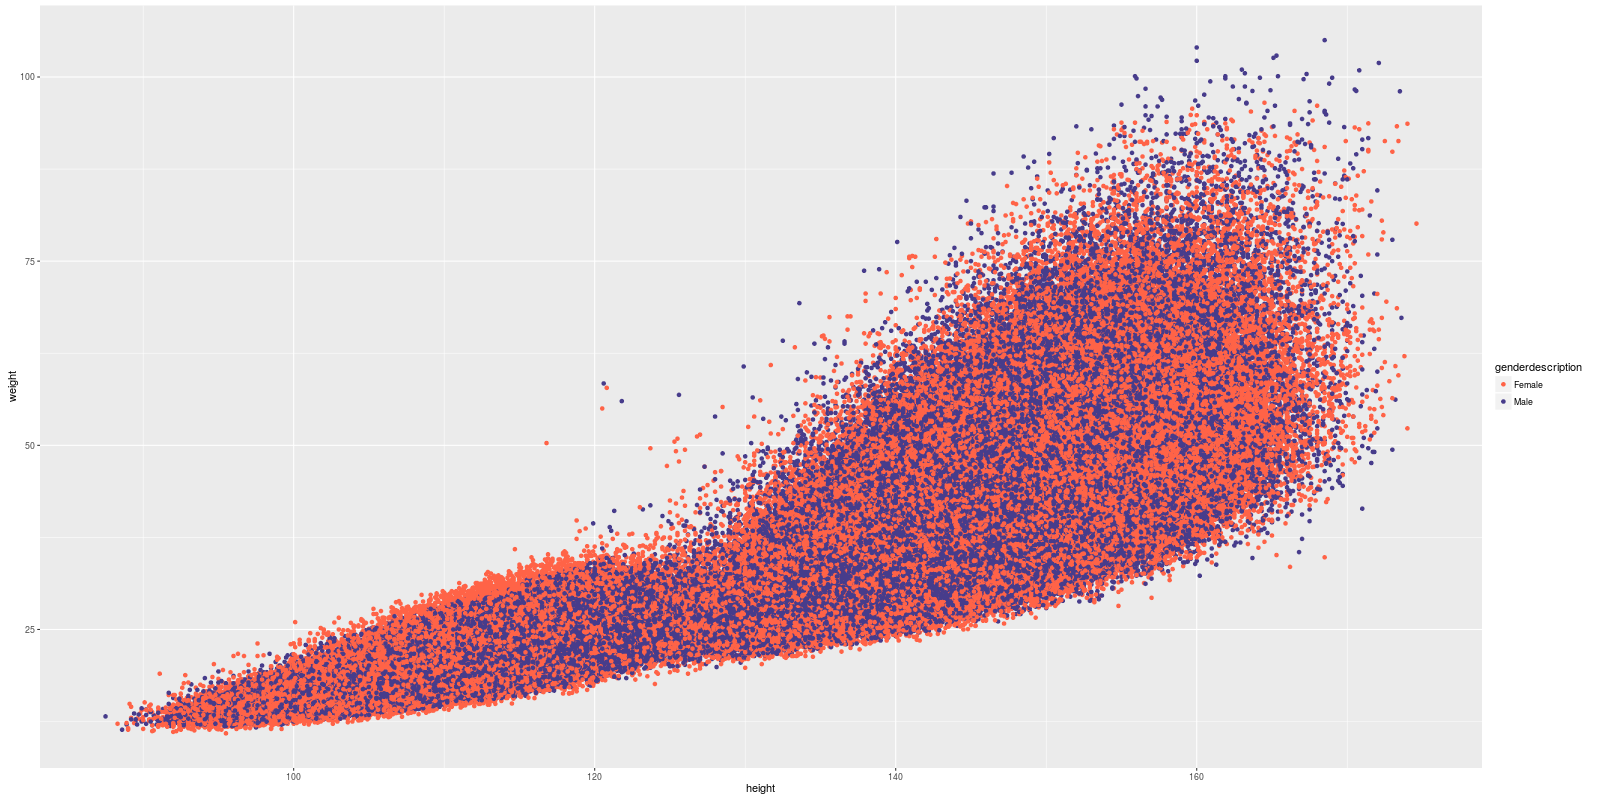
\includegraphics[scale=0.3]{heightweightgender.png}
\end{center}
\caption{Height vs weight}
\end{figure}
In the previous plot we notice the increase of height lead to increase of weight as well.
\begin{figure}[H]
	\begin{center}
		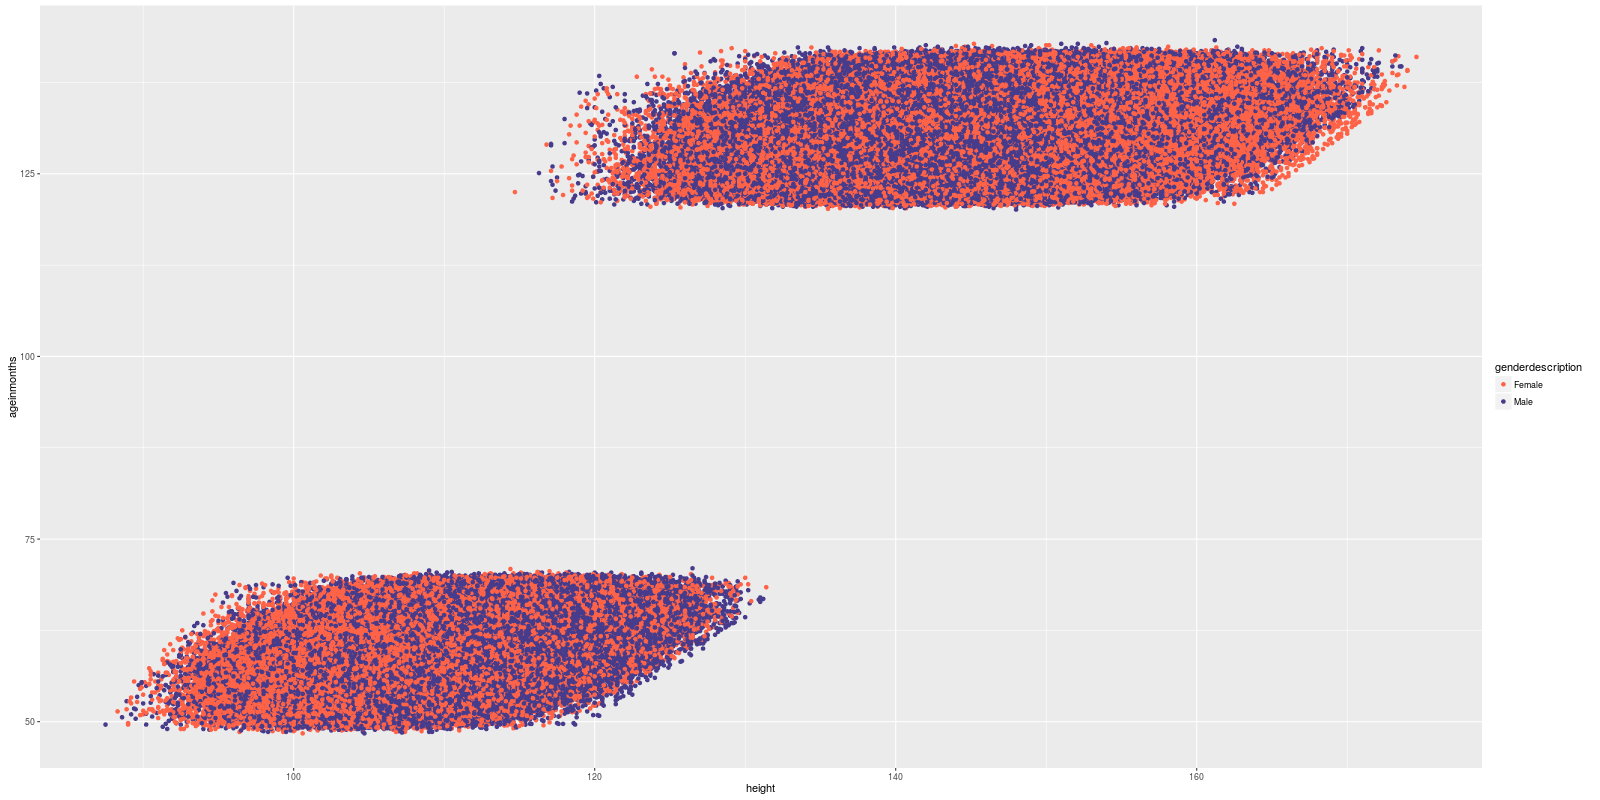
\includegraphics[scale=0.3]{heightage.png}
	\end{center}
	\caption{Height vs Age}
\end{figure}
	In this figure we notice that there is a break in the data which cause this empty area.
\begin{figure}[H]
	\begin{center}
		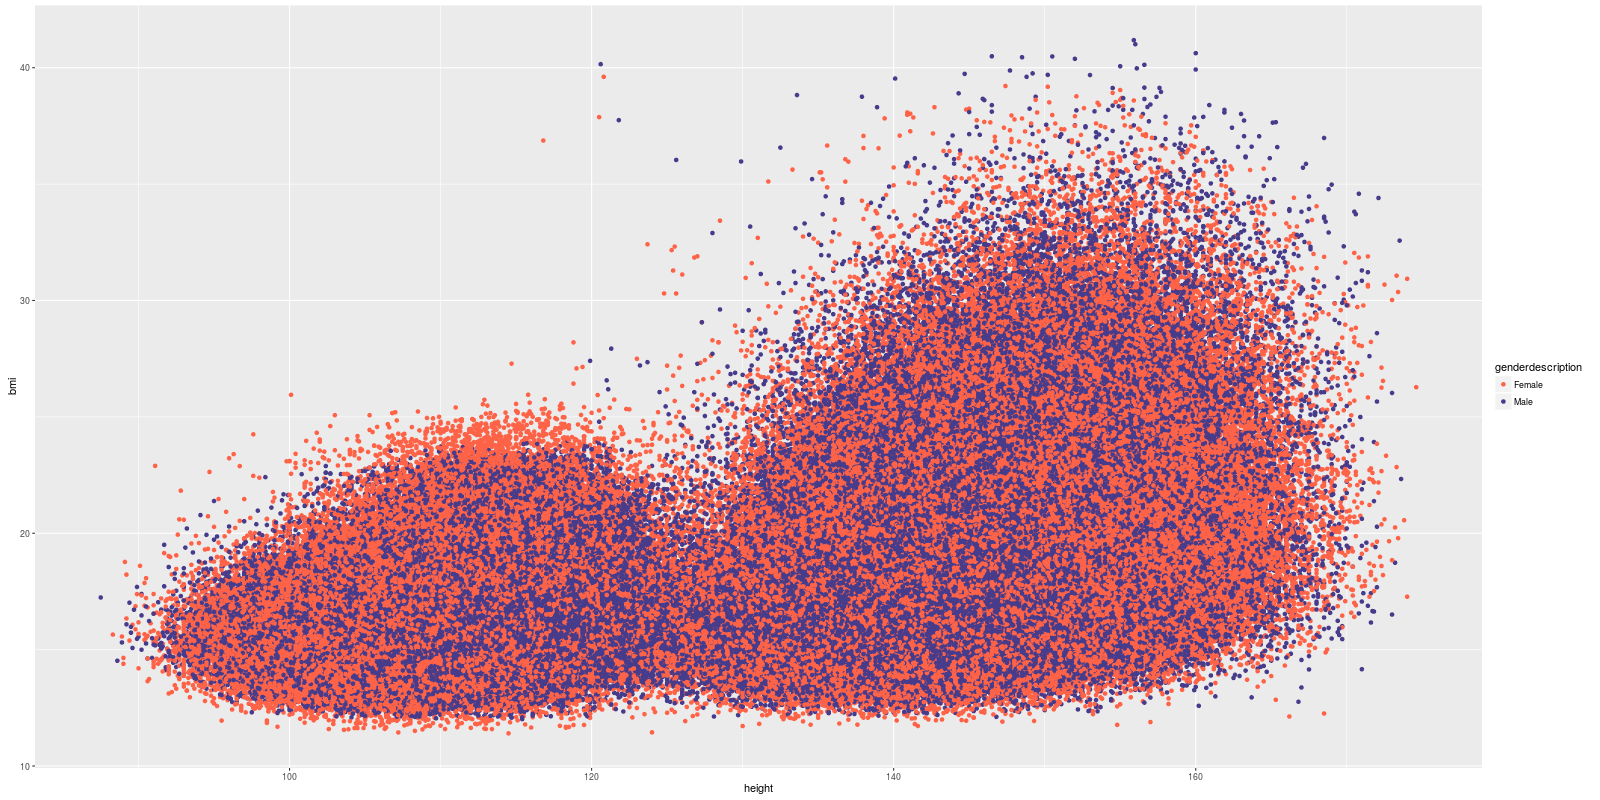
\includegraphics[scale=0.3]{heightBMI.png}
	\end{center}
	\caption{Height vs BMI}
\end{figure}
In the previous figure we notice the higher the higher BMI.
\begin{figure}[H]
	\begin{center}
		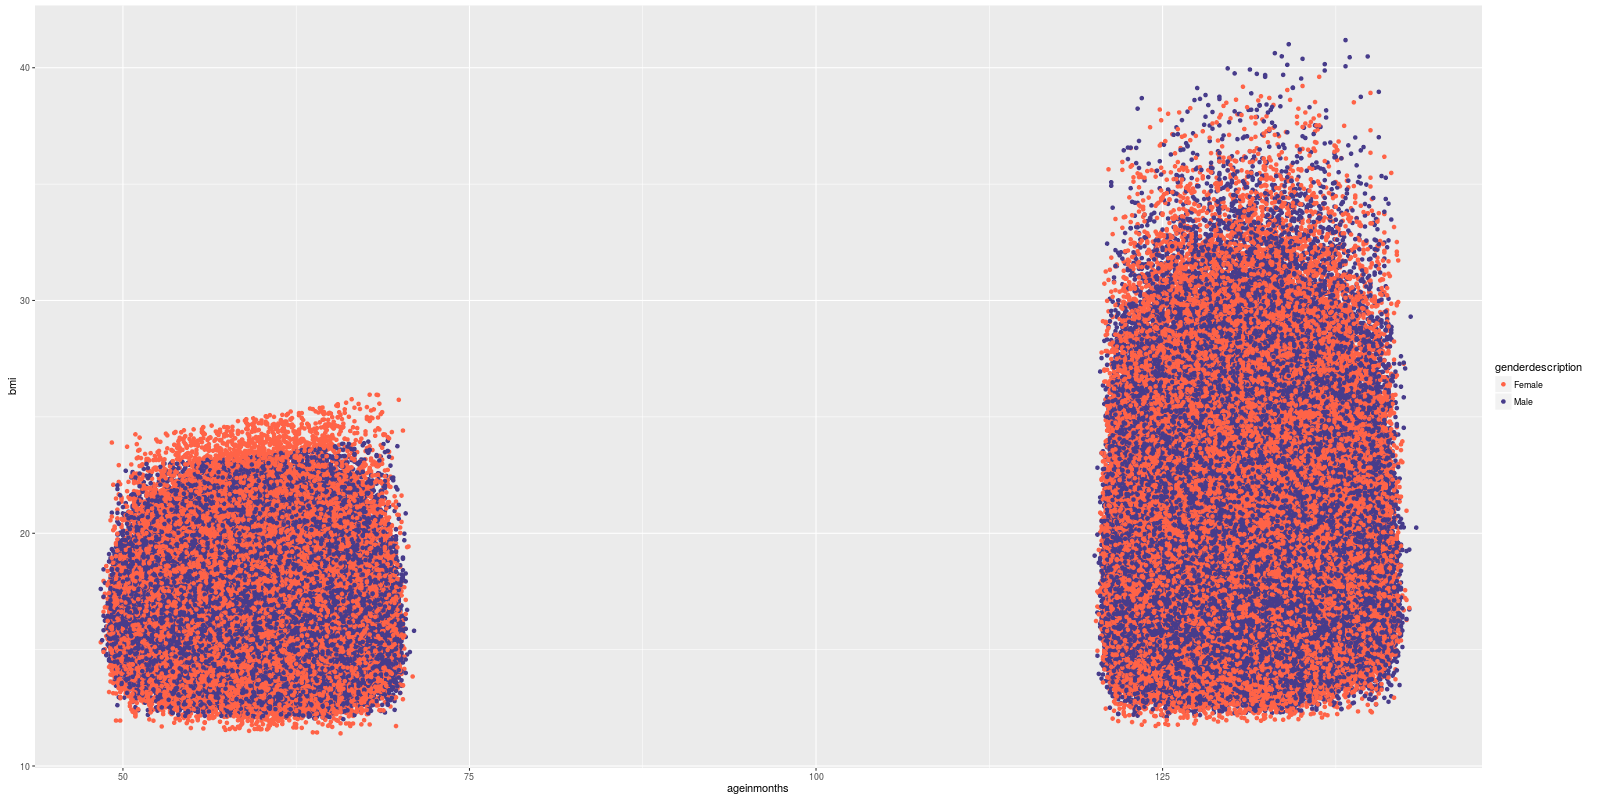
\includegraphics[scale=0.3]{ageBMI.png}
	\end{center}
	\caption{Age vs BMI}
\end{figure}
In Figure 4 we can see that we have two quantiles of ages. And the older the more BMI.
\begin{figure}[H]
	\begin{center}
		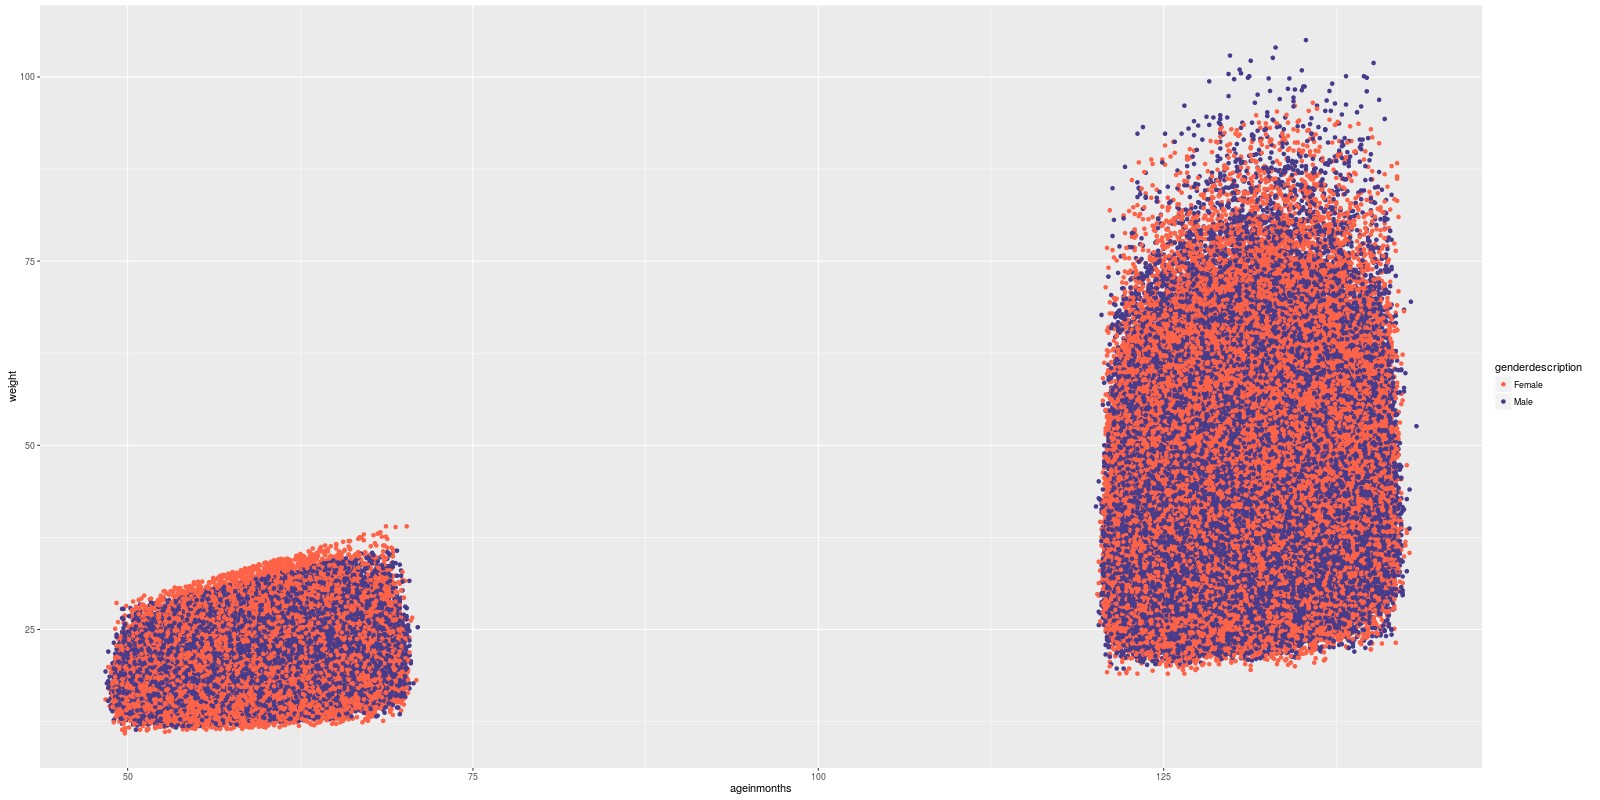
\includegraphics[scale=0.3]{ageweight.png}
	\end{center}
	\caption{Age vs weight}
\end{figure}
It's expected here where the age increase , the weight increase as well.
\begin{figure}[H]
	\begin{center}
		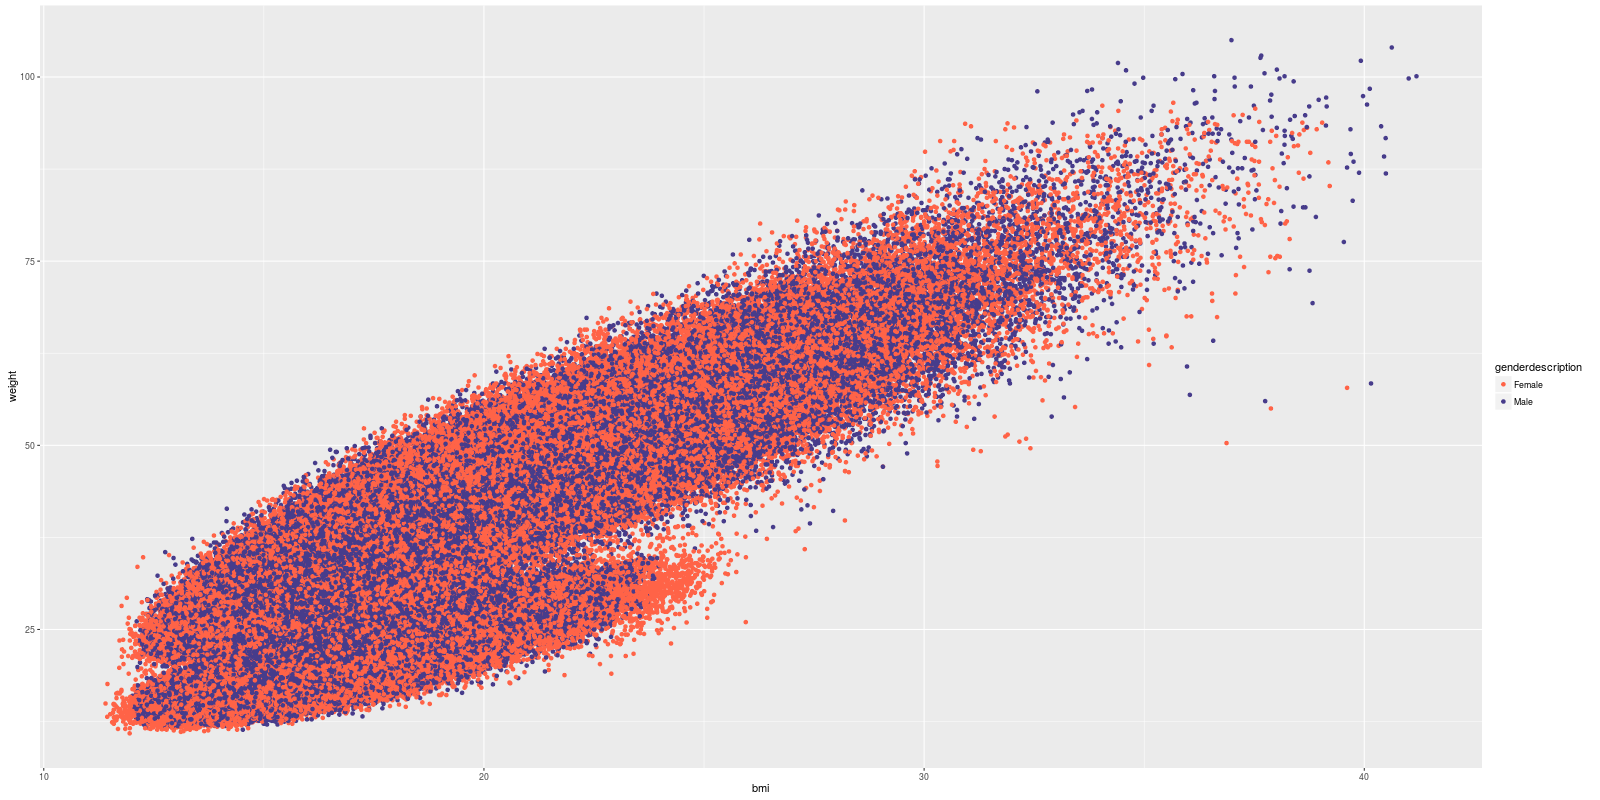
\includegraphics[scale=0.3]{BMIweight.png}
	\end{center}
	\caption{BMI vs weight}
\end{figure}
In figure 6 we can see that increasing in weight mean increase in BMI.
\(BMI = \frac{weight}{height^2}\)
\textbf{Note:}Although the previous plots looks cool (for me at least :) ) but I think there isn't much information we can get from.
To plot the previous figures I used the following code:
\begin{lstlisting}[language=R]
library(ggplot2)
#Height Weight
png('heightweight.png',height = 800,width = 1600)
qplot(height,weight,colour =genderdescription,data = ncmp)+ 
scale_color_manual(values=c("tomato", "slateblue4"))
dev.off()
# Height Age
png('heightage',height = 800,width = 1600)
qplot(height,ageinmonths,colour =genderdescription,data = ncmp)+ 
scale_color_manual(values=c("tomato", "slateblue4"))
dev.off()
# Height BMI
png('heightBMI',height = 800,width = 1600)
qplot(height,bmi,colour =genderdescription,data = ncmp)+ 
scale_color_manual(values=c("tomato", "slateblue4"))
dev.off()
# age BMI
png('ageBMI',height = 800,width = 1600)
qplot(ageinmonths,bmi,colour =genderdescription,data = ncmp)+ 
scale_color_manual(values=c("tomato", "slateblue4"))
dev.off()

# age weight
png('ageweight',height = 800,width = 1600)
qplot(ageinmonths,weight,colour =genderdescription,data = ncmp)+ 
scale_color_manual(values=c("tomato", "slateblue4"))
dev.off()

# BMI weight
png('BMIweight',height = 800,width = 1600)
qplot(bmi,weight,colour =genderdescription,data = ncmp)+ 
scale_color_manual(values=c("tomato", "slateblue4"))
dev.off()

\end{lstlisting}
In the following figure we can see the caterogical bmi of the kids depending on there age,and BMI : 
\begin{figure}[H]
	\begin{center}
		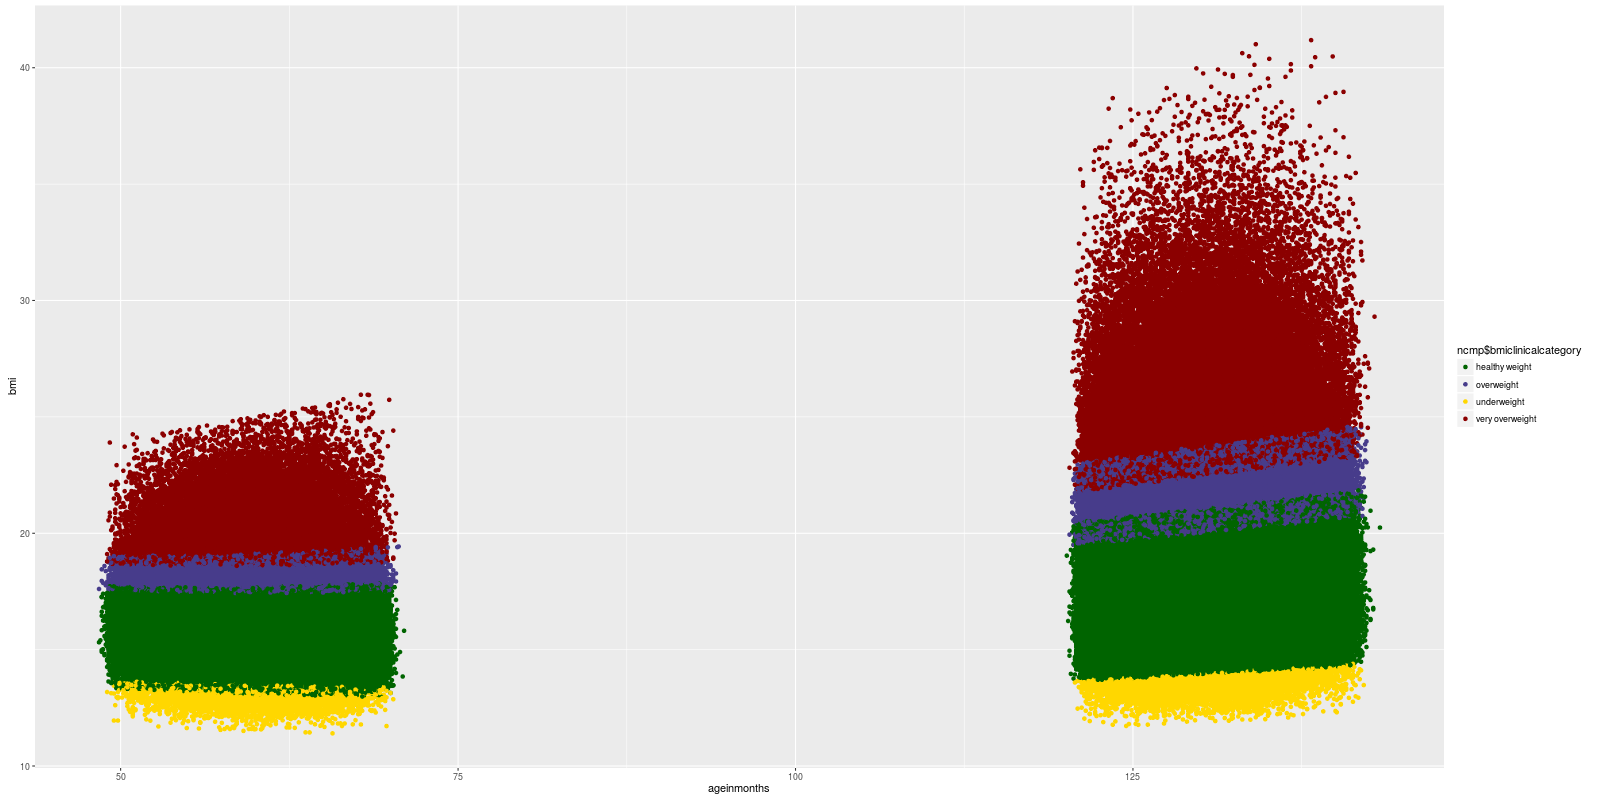
\includegraphics[scale=0.3]{bmicatage.PNG}
	\end{center}
	\caption{age vs BMI}
\end{figure}
And here is the code that generated the previous figure.
\begin{lstlisting}[language=R]
#bmi category with age
png('bmicatage',height = 800,width = 1600)
qplot(ageinmonths,bmi,colour =ncmp$bmiclinicalcategory,data = ncmp)+
scale_color_manual(values=c("darkgreen", "slateblue4","gold","darkred"))
dev.off()
\end{lstlisting}
	\section*{Third Question}
	For this question I used Mosteller formula to calculate Body Surface Area \(BSA =\frac{\sqrt{W\times H}}{60}\)
	In the following plots I colored them depending to BMI clinical category because it was continuous at some ranges. 
	\begin{figure}[H]
		\begin{center}
			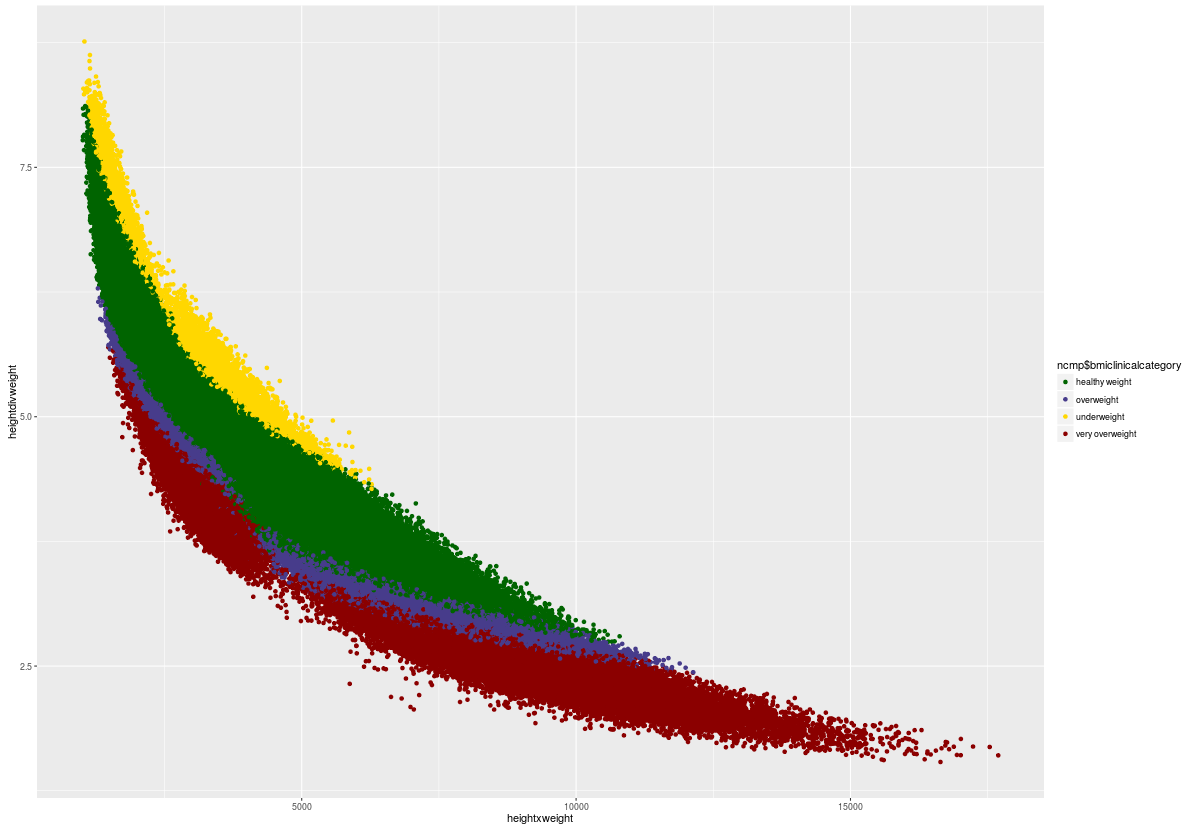
\includegraphics[scale=0.4]{xdiv.png}
		\end{center}
		\caption{Multiplication vs Devision of height and weight }
	\end{figure}
	
		\begin{figure}[H]
			\begin{center}
				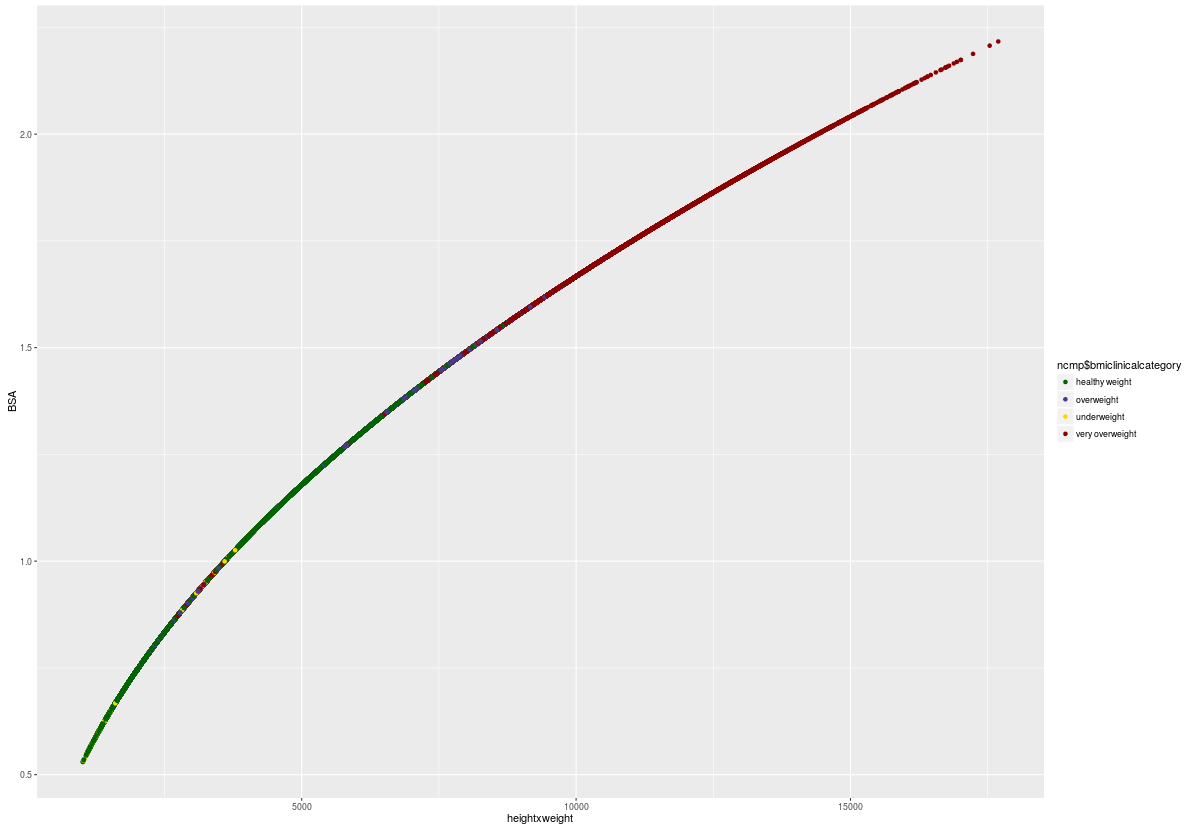
\includegraphics[scale=0.4]{xbsa.png}
			\end{center}
			\caption{Multiplication vs BSA}
		\end{figure}
				\begin{figure}[H]
					\begin{center}
						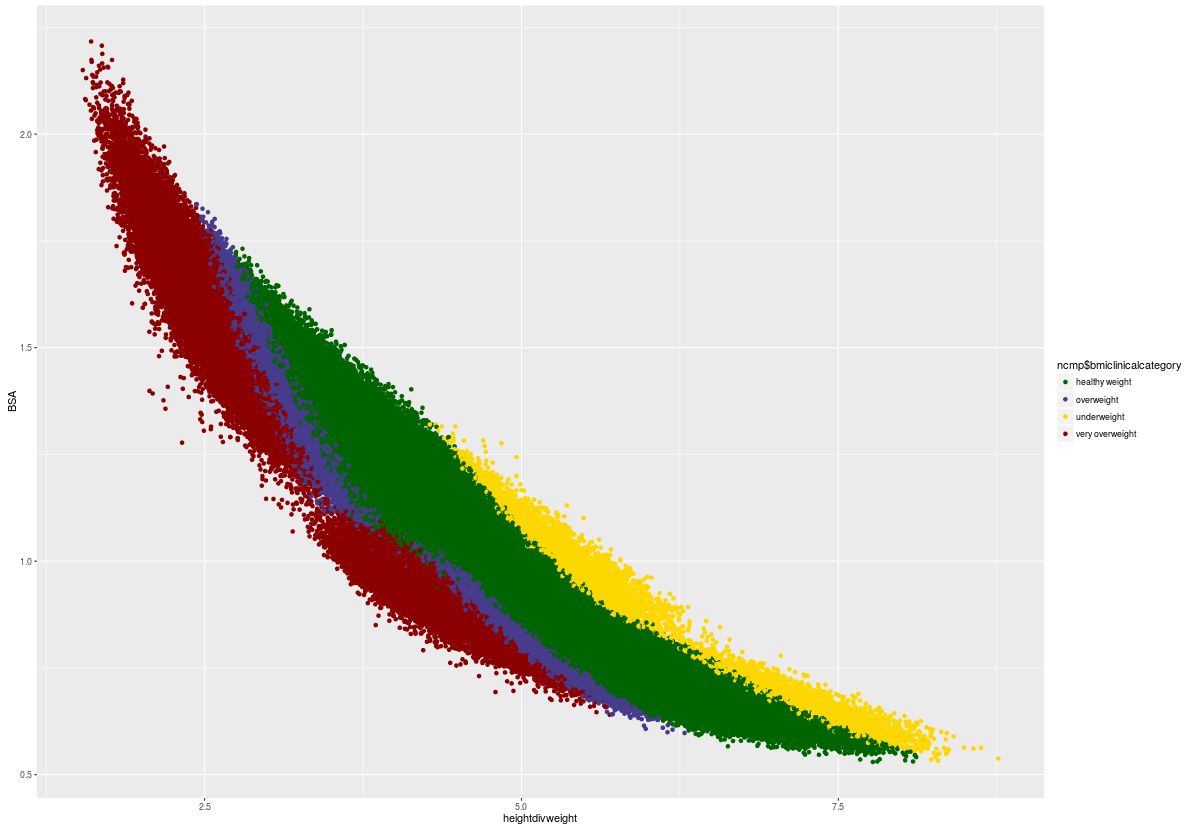
\includegraphics[scale=0.4]{divbsa.png}
					\end{center}
					\caption{Devision vs BSA}
				\end{figure}
	\section*{Fourth Question}
	\section*{Fifth Question}
	\section*{Sixth Question}
\end{document}